%% 
%% Copyright 2007-2020 Elsevier Ltd
%% 
%% This file is part of the 'Elsarticle Bundle'.
%% ---------------------------------------------
%% 
%% It may be distributed under the conditions of the LaTeX Project Public
%% License, either version 1.2 of this license or (at your option) any
%% later version.  The latest version of this license is in
%%    http://www.latex-project.org/lppl.txt
%% and version 1.2 or later is part of all distributions of LaTeX
%% version 1999/12/01 or later.
%% 
%% The list of all files belonging to the 'Elsarticle Bundle' is
%% given in the file `manifest.txt'.
%% 
%% Template article for Elsevier's document class `elsarticle'
%% with harvard style bibliographic references

%\documentclass[preprint,12pt,authoryear]{elsarticle}

%% Use the option review to obtain double line spacing
%% \documentclass[authoryear,preprint,review,12pt]{elsarticle}

%% Use the options 1p,twocolumn; 3p; 3p,twocolumn; 5p; or 5p,twocolumn
%% for a journal layout:
%% \documentclass[final,1p,times,authoryear]{elsarticle}
%% \documentclass[final,1p,times,twocolumn,authoryear]{elsarticle}
%% \documentclass[final,3p,times,authoryear]{elsarticle}
%% \documentclass[final,3p,times,twocolumn,authoryear]{elsarticle}
%% \documentclass[final,5p,times,authoryear]{elsarticle}
 \documentclass[final,5p,times,twocolumn,authoryear]{elsarticle}

%% For including figures, graphicx.sty has been loaded in
%% elsarticle.cls. If you prefer to use the old commands
%% please give \usepackage{epsfig}

%% The amssymb package provides various useful mathematical symbols
\usepackage{amssymb}
\usepackage{lipsum}
%% The amsthm package provides extended theorem environments
%% \usepackage{amsthm}

%% The lineno packages adds line numbers. Start line numbering with
%% \begin{linenumbers}, end it with \end{linenumbers}. Or switch it on
%% for the whole article with \linenumbers.
%% \usepackage{lineno}

%% You might want to define your own abbreviated commands for common used terms, e.g.:
\newcommand{\kms}{km\,s$^{-1}$}
\newcommand{\msun}{$M_\odot}

\journal{Results in Physics}


\begin{document}

\begin{frontmatter}

%% Title, authors and addresses

%% use the tnoteref command within \title for footnotes;
%% use the tnotetext command for theassociated footnote;
%% use the fnref command within \author or \affiliation for footnotes;
%% use the fntext command for theassociated footnote;
%% use the corref command within \author for corresponding author footnotes;
%% use the cortext command for theassociated footnote;
%% use the ead command for the email address,
%% and the form \ead[url] for the home page:
%% \title{Title\tnoteref{label1}}
%% \tnotetext[label1]{}z
%% \author{Name\corref{cor1}\fnref{label2}}
%% \ead{email address}
%% \ead[url]{home page}
%% \fntext[label2]{}
%% \cortext[cor1]{}
%% \affiliation{organization={},
%%            addressline={}, 
%%            city={},
%%            postcode={}, 
%%            state={},
%%            country={}}
%% \fntext[label3]{}

\title{A Game Theory Simulation on the Battle of Gettysburg using Agent-Based-Modeling}
%% use optional labels to link authors explicitly to addresses:
%% \author[label1,label2]{}
%% \affiliation[label1]{organization={},
%%             addressline={},
%%             city={},
%%             postcode={},
%%             state={},
%%             country={}}
%%
%% \affiliation[label2]{organization={},
%%             addressline={},
%%             city={},
%%             postcode={},
%%             state={},
%%             country={}}

\author{Rubén Hernández O'kelly}
\affiliation{organization={Institute for Computing in Research},
            city={Santa Fe}, 
            state={NM},
            postcode={2023}}

\begin{abstract}
%% Text of abstract
This paper intends to find the difference between the Battle of Gettysburg, an important battle of the American Civil War, and an agent-based simulation of the battle using the principles of Game Theory as basis for the agents' decisions. In this simulation, the Union will be the main focus. As the simulation ends, the two results will be compared and will show the best actions that the Union could have made.
\end{abstract}

%%Graphical abstract
%\begin{graphicalabstract}
%\includegraphics{grabs}
%\end{graphicalabstract}

%%Research highlights
%\begin{highlights}
%\item Research highlight 1
%\item Research highlight 2
%\end{highlights}

\begin{keyword}
%% keywords here, in the form: keyword \sep keyword, up to a maximum of 6 keywords
Game Theory \sep Agent-based modeling \sep Simulation \sep Gettysburg

%% PACS codes here, in the form: \PACS code \sep code

%% MSC codes here, in the form: \MSC code \sep code
%% or \MSC[2008] code \sep code (2000 is the default)

\end{keyword}


\end{frontmatter}

%\tableofcontents

%% \linenumbers

%% main text

\section{Introduction}
\label{introduction}

“Let your plans be dark and impenetrable as night, and when you move, fall like a thunderbolt.”
― Sun Tzu, The Art of War. Sun Tzu's quote epitomizes the significance of secrecy and surprise in warfare. In the context of the Battle of Gettysburg and the project's exploration of game theory and agent-based modeling, it emphasizes the importance of uncertainty and adaptive decision-making by the generals. Employing this strategic philosophy, simulated agents in agent-based modeling can replicate the challenges faced by real generals, allowing for a deeper understanding of the battle's complex dynamics.

\section{Scenario and Methodology}
%%\label{}
%%\subsection{Backgrounds}

The Battle of Gettysburg, fought from July 1 to July 3, 1863, during the American Civil War, was a pivotal and bloody conflict between the Union Army of the Potomac, commanded by General George G. Meade, and the Confederate Army of Northern Virginia, led by General Robert E. Lee. It took place in the small town of Gettysburg, Pennsylvania, and is often considered the turning point of the Civil War. The battle was a result of Lee's second invasion of the North and his attempt to gain a strategic advantage by taking the war to Union territory. The three-day battle saw intense fighting and heavy casualties on both sides, with approximately 51,000 soldiers killed, wounded, or missing. The Union emerged victorious, and Lee's Confederate forces were forced to retreat back to Virginia, effectively ending the South's hopes for a successful invasion of the North.

The Battle of Gettysburg is renowned for its significance in the Civil War's outcome and its impact on American history. The Union victory boosted Northern morale and solidified President Abraham Lincoln's resolve to issue the Emancipation Proclamation later that year, declaring the freedom of all slaves in Confederate-held territories. Furthermore, the battle prompted Lee to abandon future offensives in the North, shifting the focus of the war to Virginia and eventually leading to the Union's triumph.

Game theory is a branch of mathematics and economics that deals with strategic interactions among multiple decision-makers (players) who aim to maximize their utility or payoff (rewards). It provides a formal framework to analyze and predict how individuals or organizations make decisions in competitive situations. Developed in the mid-20th century, game theory has found applications in various fields, including economics, political science, biology, and computer science. The central concept in game theory is the "game," which consists of players, strategies, and payoffs. Different games, such as Prisoner's Dilemma, Battle of the Sexes, and Chicken, present various scenarios of conflict, cooperation, and decision-making, offering valuable insights into real-world situations.

Agent-Based Modeling (ABM) is a computational modeling technique used to simulate the behavior and interactions of individual agents to understand complex systems' emergent properties. In ABM, agents are autonomous entities that follow predefined rules and adapt their behavior based on their local environment and interactions with other agents. The model's dynamics emerge from the collective behavior of these agents, allowing researchers to observe and analyze the system's macro-level patterns and outcomes. ABM has gained popularity across various domains, including sociology, ecology, economics, and epidemiology, as it provides a powerful tool to study systems that involve numerous autonomous agents and complex interactions. ABM allows researchers to explore "what-if" scenarios, test hypotheses, and gain insights into the system's behavior that may not be apparent through traditional analytical methods.

\section{Methods and Results}
%%\label{}
The simulation results will be compared to the historical outcome of the Battle of Gettysburg to identify effective strategies that the Union could have employed. By applying game theory principles and agent-based modeling, we hope to gain valuable insights into the decision-making dynamics of this critical historical event. 

To conduct the agent-based simulation, we developed a Python program that models the Battle of Gettysburg using game theory principles. The simulation involves two teams, the Union and the Confederacy, each represented by agents with unique characteristics such as health, attack range, and attack strength. The agents follow predefined rules and adapt their actions based on their local environment and interactions with other agents.

The simulation progresses through a series of steps, with each step representing a moment in the battle. At each step, the agents make decisions on whether to attack enemy agents within their attack range or to retreat to a common point for regrouping. The agents' strategies are based on the principles of game theory, seeking to maximize their utility (in this case, winning the battle) while anticipating the opponents' actions.

Upon completion of the simulation, we compare the results with the historical outcome of the Battle of Gettysburg. We evaluate the effectiveness of different strategies employed by the Union agents and identify potential improvements in their decision-making. The findings shed light on the significance of adaptive decision-making and the impact of uncertainty on battle outcomes.

The program is conducted in such a way that the agents are arranged by formations which resemble those used in the actual battle:

\begin{figure}[!ht]
  \centering
      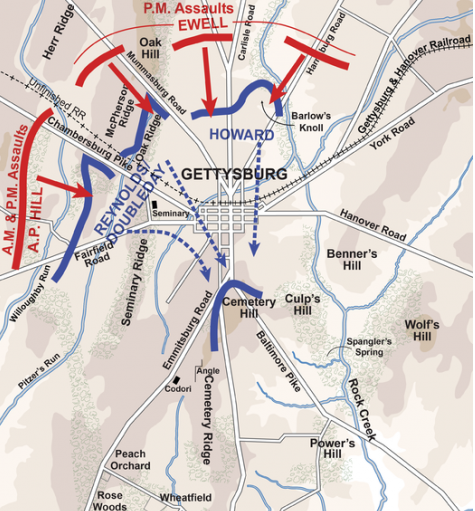
\includegraphics[width=6cm]{Gettysburg_map.png}
      \caption{The map of the Battle of Gettysburg}
      \label{fig:Map}
  \centering
\end{figure}

\begin{figure}[!ht]
  \centering
      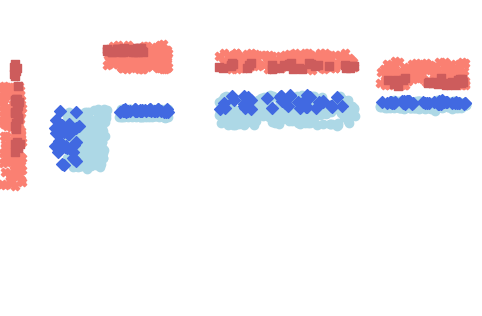
\includegraphics[width=6cm]{sim_gett_map.png}
      \caption{A simulated map of the Battle of Gettysburg}
      \label{fig:Map}
  \centering
\end{figure}

The simulation has been run dozens of times to fully grasp the aspect of unique decision-making by the agents. Although each time has been unique,  

\section{Summary and conclusions}
%%\label{}
\lipsum[1-4]


\section*{Acknowledgements}
Thanks to ...

%% The Appendices part is started with the command \appendix;
%% appendix sections are then done as normal sections
\appendix

\section{Appendix title 1}
%% \label{}

\section{Appendix title 2}
%% \label{}

%% If you have bibdatabase file and want bibtex to generate the
%% bibitems, please use
%%
\bibliographystyle{elsarticle-harv} 
\bibliography{example}

%% else use the following coding to input the bibitems directly in the
%% TeX file.

%%\begin{thebibliography}{00}

%% \bibitem[Author(year)]{label}
%% For example:

%% \bibitem[Aladro et al.(2015)]{Aladro15} Aladro, R., Martín, S., Riquelme, D., et al. 2015, \aas, 579, A101


%%\end{thebibliography}

\end{document}

\endinput
%%
%% End of file `elsarticle-template-harv.tex'.
